\documentclass{article}
\usepackage[utf8]{vietnam}
\usepackage{graphicx}
\begin{document}
%%%%%%%%%%%%%%%%%%%%%%%%%%%%%%%%%%%%%
% \section{Trang bìa}
% \begin{titlepage}
\begin{tikzpicture}[remember picture, overlay]
\draw [line width = 3pt]
($ (current page.north west) + (3.0cm, - 2.5cm)$)
rectangle
($ (current page.south east) + (- 2.5cm, 2.5cm)$);
\draw [line width = 0.5pt]
($ (current page.north west) + (3.1cm, - 2.6cm)$)
rectangle
($ (current page.south east) + (- 2.6cm, 2.6cm)$);
\end{tikzpicture}
\begin{center}
\vspace{- 0.4cm}
\textbf{ĐẠI HỌC BÁCH KHOA HÀ NỘI} \\
\textbf{VIỆN TOÁN ỨNG DỤNG VÀ TIN HỌC} \\
\textbf{******}
\vspace{0.8cm}

\begin{figure}[h]
\centering

\includegraphics[scale = .5]{pictures/logoBK.png}
\end{figure}
\vspace{0.7cm}
\textbf{\fontsize{16pt}{30pt}\selectfont {BÁO CÁO ĐỒ ÁN II}} \\
\vspace{1cm}
\textbf{\fontsize{20pt}{24pt}\selectfont {ĐỀ TÀI:}} \\
\textbf{\fontsize{19pt}{24pt}\selectfont {Xây dựng kiến trúc vi dịch vụ cho bài toán hóa đơn điện tử}} \\
% \textbf{\fontsize{20pt}{24pt}\selectfont {Sử dụng thiết kế hướng miền xây dựng kiến trúc vi dịch vụ cho bài toán hóa đơn điện tử}} \\
\end{center}
\vspace{0.7cm}

\hspace{2.4cm}
\begin{minipage}{0.8\textwidth}
\textbf{Giảng viên hướng dẫn: TS. Vũ Thành Nam}
\end{minipage}

\hspace{3cm}
\begin{minipage}{0.7\textwidth}
\begin{tabular}{l l l}
Sinh viên thực hiện & Vũ Văn Nghĩa \\
Mã số sinh viên & 20206205 \\
Lớp & Toán Tin 02 - K65 \\
\end{tabular}
\end{minipage}

\hspace{2.4cm}
\begin{center}
\textbf{\fontsize{20pt}{24pt}\selectfont {Chuyên ngành: Toán Tin}}
\end{center}

\vspace{0.5cm}
\begin{center}
\textbf{Hà Nội, \the\month - \the\year}
\end{center}
\end{titlepage}

% \newpage
% \thispagestyle{empty}

% \section{Nhận xét của giảng viên}
% \newpage

\begin{center}
{\bfseries NHẬN XÉT CỦA GIẢNG VIÊN HƯỚNG DẪN}
\end{center}

\begin{enumerate}
\item Mục đích và nội dung của đồ án:
\vspace{20ex} % Thêm khoảng cách dọc
\item 	Kết quả đạt được:
\vspace{20ex} % Thêm khoảng cách dọc
\item 	Ý thức làm việc của sinh viên:
\vspace{20ex} % Thêm khoảng cách dọc
\end{enumerate}

\hspace{0.4\textwidth}
\begin{minipage}{0.5\textwidth}
\noindent\begin{center}
\textit{Hà Nội, \today} \\
\textbf{Giảng viên hướng dẫn} \\
\textit{(Ký và ghi rõ họ tên)}
\end{center}
\end{minipage}

\pagestyle{empty}

\newpage


% \section{Mục lục}
% \tableofcontents

% \section{Lời cảm ơn}
% \newpage

\section*{\centering LỜI CẢM ƠN}

\addcontentsline{toc}{section}{LỜI CẢM ƠN}

\newpage



% \section{Lời mở đầu}
% \newpage

\section*{\centering LỜI MỞ ĐẦU}

\addcontentsline{toc}{section}{LỜI MỞ ĐẦU}

\newpage

% \section{Tóm tắt nội dung đồ án}
% \newpage
\section*{\centering TÓM TẮT NỘI DUNG ĐỒ ÁN}
\addcontentsline{toc}{section}{TÓM TẮT NỘI DUNG ĐỒ ÁN}
\newpage

% \section{Đánh giá và thảo luận}
% \newpage
\section*{\centering ĐÁNH GIÁ VÀ THẢO LUẬN}
\addcontentsline{toc}{section}{ĐÁNH GIÁ VÀ THẢO LUẬN}
\newpage

% \section{Danh sách bảng}
% \section{Danh sách hình ảnh}
% \section{Danh sách mã nguồn}

% \section{Danh sách các cụm từ viết tắt}
% \newpage
\section*{\centering DANH SÁCH CÁC CỤM TỪ VIẾT TẮT}
\addcontentsline{toc}{section}{DANH SÁCH CÁC CỤM TỪ VIẾT TẮT}

% @sau

\begin{table}[h]
\centering
\begin{tabular}{|c|c|c|c|}
\hline
STT & Từ viết tắt & Từ viết đầy đủ & Mô tả \\
\hline
Dong1 & Dong1 & Cot1 & Cot2 \\
\hline
Dong2 & Dong2 & Cot1 & Cot2 \\
\hline
\end{tabular}
\caption{ViDuBangThuong}
\end{table}

\newpage

% API; Application Programming Interface; Giao diện lập trình ứng dụng
% CI/CD; Continuous Integration (CI) and Continuous Delivery (CD) ; Quá trình tích hợp và chuyển giao liên tục
% thiết kế hướng miền ; thiết kế hướng miền; Kỹ thuật thiết kế theo hướng miền
% DI; Dependency Injection; Cơ chế tiêm sự phụ thuộc giữa các đối tượng
% HTTP; Hypertext Transfer Protocol; Giao thức truyền tải siêu văn bản
% JSON; JavaScript Object Notation; Một kiểu dữ liệu mở rộng của JavaScript
% ORM; Object Relational Mapping; Một kỹ thuật ánh xạ các đối tượng lập trình với từng bảng trong CSDL quan hệ
% Cơ sở dữ liệu ; CSDL ;
% Tạo (Create), Đọc (Read), Sửa (Update), Xóa (Delete) ; CRUD ;
% Kubernetes ; K8s ; kubernetes
% Số điện thoại ; SĐT ;
% UML
% MVC; Model View Controller; Một mẫu thiết kế ứng dụng
% SQL

SOA; Service Oriented Architecture; Kiến trúc hướng dịch vụ
SOAP; Simple Object Access Protocol; Một giao thức để truy cập dịch vụ web
SPA; Single Page Application; Kiểu ứng dụng một trang
REST; Representational State Transfer; Một tiêu chuẩn thiết kế các API sử dụng cho các dịch vụ web
URL; Uniform Resource Locator ; Địa chỉ định vị tài nguyên trên Internet
XML; Extensible Markup Language; Ngôn ngữ đánh dấu mở rộng

% TCT ; TCT ;
Người nộp thuế ; NNT ;
Mã số thuế ; MST ;
Hóa đơn điện tử ; HĐĐT ;
Cơ quan thuế ; CQT ;
Công nghệ thông tin ; CNTT ;



% \section{Danh sách các thuật ngữ}
% % STT; Tiếng Anh; Tiếng Việt
% @sau

% kiến trúc nguyên khối, kiến trúc nguyên khối
% kiến trúc nguyên khối, kiến trúc nguyên khối
% kiến trúc vi dịch, kiến trúc vi dịch
% kiến trúc vi dịch, kiến trúc vi dịch
% kiến trúc vi dịch, kiến trúc vi dịch
% kiến trúc vi dịch, kiến trúc vi dịch
% thiết kế hướng miền, thiết kế hướng miền
% thiết kế hướng miền, thiết kế hướng miền

1 thiết kế hướng miền
Thiết kế hướng lĩnh vực
2 Domain (không dịch)
3 Abstraction Trừu tượng
4 chuyên gia ngành

%%%%%%%%%%%
% \section{Giới thiệu}
% Trong thời đại ngày nay, nhu cầu phát triển ứng dụng và hệ thống ngày càng tăng, đặt ra thách thức đối với kiến trúc phần mềm. Kiến trúc nguyên khối đã phục vụ hiệu quả trong quá khứ, nhưng kiến trúc này bắt đầu gặp khó khăn đối mặt với sự phức tạp, khả năng mở rộng và khả năng đáp ứng linh hoạt với thay đổi nhanh chóng trong yêu cầu kinh doanh.

Kiến trúc vi dịch vụ là giải pháp cho những thách thức trên. Kiến trúc vi dịch vụ chia dự án thành những dịch vụ nhỏ độc lập, mỗi dịch vụ chịu trách nhiệm về một chức năng cụ thể. Từ đó, giảm sự phức tạp của dự án tăng tính linh hoạt và dễ dàng quản lý.

Việc vận dụng kết hợp giữa kiến trúc vi dịch vụ và thiết kế hướng miền là một cách tiếp cận toàn diện, giúp xác định và tổ chức các dịch vụ dựa trên việc hiểu rõ về lĩnh vực kinh doanh. Thiết kế hướng miền xây dựng mô hình dựa trên yêu cầu nghiệp vụ thực tế, từ đó dự án phản ánh đúng các quy trình kinh doanh.

% \subsection{Giới thiệu về bài toán hóa đơn điện tử}
% Bài toán hóa đơn điện tử là một phần quan trọng của quá trình chuyển đổi số. Trong quá khứ, mọi người thường sử dụng hóa đơn giấy truyền thống. Ngày nay, khi có quy định kế toán và quản lý tài chính, hóa đơn điện tử đã trở nên phổ biến giúp giảm bớt sự phụ thuộc vào giấy tờ. Cùng với sự phát triển của khoa học công nghệ đã giúp quản lí hiệu quả công việc và tối ưu hóa quy trình kế toán và tài chính.

Theo em tìm hiểu có các khái niệm và căn cứ pháp lý liên quan sau đây:

% \subsubsection{Hóa đơn}
% %%%%%%%%%%%%%%%%%%%%%%%%%%%%%%%%%%%%%!

Hóa đơn là chứng từ kế toán do tổ chức, cá nhân bán hàng hóa, cung cấp dịch vụ lập, ghi nhận thông tin bán hàng hóa, cung cấp dịch vụ. Hóa đơn được thể hiện theo hình thức hóa đơn điện tử hoặc hóa đơn do cơ quan thuế đặt in.

%%%%%%%%%%%%%%%%%%%%%%%%%%%%%%%%%%%%%!



% \subsubsection{Hóa đơn điện tử}
% Hóa đơn điện tử là hóa đơn có mã hoặc không có mã của cơ quan thuế được thể hiện ở dạng dữ liệu điện tử do tổ chức, cá nhân bán hàng hóa, cung cấp dịch vụ lập bằng phương tiện điện tử để ghi nhận thông tin bán hàng hóa, cung cấp dịch vụ theo quy định của pháp luật về kế toán, pháp luật về thuế, bao gồm cả trường hợp hóa đơn được khởi tạo từ máy tính tiền có kết nối chuyển dữ liệu điện tử với cơ quan thuế, trong đó:

a. Hóa đơn điện tử có mã của cơ quan thuế là hóa đơn điện tử được cơ quan thuế cấp mã trước khi tổ chức, cá nhân bán hàng hóa, cung cấp dịch vụ gửi cho người mua. Mã của cơ quan thuế trên hóa đơn điện tử bao gồm số giao dịch là một dãy số duy nhất do hệ thống của cơ quan thuế tạo ra và một chuỗi ký tự được cơ quan thuế mã hóa dựa trên thông tin của người bán lập trên hóa đơn.

b. Hóa đơn điện tử không có mã của cơ quan thuế là hóa đơn điện tử do tổ chức bán hàng hóa, cung cấp dịch vụ gửi cho người mua không có mã của cơ quan thuế.

% \subsubsection{Bắt buộc sử dụng hóa đơn điện tử từ 01/07/2022}
% Nghị định này có hiệu lực thi hành kể từ ngày 01 tháng 7 năm 2022, khuyến khích cơ quan, tổ chức, cá nhân đáp ứng điều kiện về hạ tầng công nghệ thông tin áp dụng quy định về hóa đơn, chứng từ điện tử của Nghị định này trước ngày 01 tháng 7 năm 2022.

% Chủ đề

Theo quy định, tất cả các doanh nghiệp, tổ chức và hộ kinh doanh đều bắt buộc phải chuyển từ sử dụng hóa đơn giấy sang hóa đơn điện tử bắt đầu từ tháng 07/2022. Vì vậy, nhu cầu sử dụng và xử lý hóa đơn điện tử trở nên rất lớn. Do đó ở đồ án này, em chọn chủ đề về quản lý hóa đơn điện tử.

% \subsubsection{Bản thể hiện của hóa đơn điện tử}
% \input{contents/ban_the_hien_cua_hoa_don_dien_tu}

% \subsubsection{Lưu trữ hóa đơn điện tử}
% Thời gian?
% 
 
\textbf{Theo quy định tại khoản 1 Điều 11 Thông tư 32/2011/TT-BTC:} 




 
  

  Người bán, người mua hàng hoá, dịch vụ sử dụng hóa đơn điện tử để ghi sổ kế toán, lập báo cáo tài chính phải lưu trữ hóa đơn điện tử theo thời hạn quy định của Luật Kế toán. Trường hợp hóa đơn điện tử được khởi tạo từ hệ thống của tổ chức trung gian cung cấp giải pháp hóa đơn điện tử thì tổ chức trung gian này cũng phải thực hiện lưu trữ hóa đơn điện tử theo thời hạn nêu trên.
  
\textbf{Theo quy định tại khoản 5 Điều 41 Luật số 88/2015/QH13:} 

  
  1. Tài liệu kế toán phải được lưu trữ theo thời hạn sau đây:
  
  a. Ít nhất là 05 năm đối với tài liệu kế toán dùng cho quản lý, điều hành của đơn vị kế toán, gồm cả chứng từ kế toán không sử dụng trực tiếp để ghi sổ kế toán và lập báo cáo tài chính.
  
  b. Ít nhất là 10 năm đối với chứng từ kế toán sử dụng trực tiếp để ghi sổ kế toán và lập báo cáo tài chính, sổ kế toán và báo cáo tài chính năm, trừ trường hợp pháp luật có quy định khác.
  
  c. Lưu trữ vĩnh viễn đối với tài liệu kế toán có tính sử liệu, có ý nghĩa quan trọng về kinh tế, an ninh, quốc phòng.
  
  => Như vậy, hóa đơn điện tử dạng tệp XML sẽ được lưu trữ trên hệ thống hóa đơn điện tử của nhà cung cấp hoặc doanh nghiệp có thể tải về để tự lưu trữ. Thời gian lưu trữ là 10 năm theo quy định của pháp luật.
  

% \subsubsection{Một số lợi ích của hóa đơn điện tử}
% Giúp tiết kiệm chi phí in ấn, lưu trữ và bảo quản.
Loại bỏ rủi ro cháy, hỏng hoặc mất và dễ dàng sao lưu.
Dễ dàng linh hoạt trong việc tra cứu, phát hành, quản lý và tạo báo cáo.
Tối ưu hóa quá trình kế toán (giảm sai sót và tiết kiệm thời gian) và giảm thủ tục giấy tờ.
Theo dõi tình hình tài chính của công ty (doanh thu, chi phí, lợi nhuận).
Tuân thủ các quy định về thuế và pháp luật.
Thể hiện tính minh bạch trong quá trình kinh doanh (bảo vệ quyền lợi của cả người mua và người bán).

% \subsection{Giới thiệu về kiến trúc vi dịch vụ}
% \subsubsection{Kiến trúc nguyên khối}
% Trước khi kiến trúc vi dịch vụ trở nên phổ biến, kiến trúc nguyên khối đã được áp dụng rộng rãi trong kiến trúc phần mềm truyền thống. Kiến trúc nguyên khối là kiến trúc phần mềm trong đó  tất cả các thành phần      của  dự án    được xây dựng thành một đơn vị triển khai    duy nhất. 

% Trong kiến trúc nguyên khối, bất kỳ thay đổi nào đối với một thành phần     đều yêu cầu toàn bộ ứng dụng phải được     kiểm thử   và triển khai lại. 




Điều này có thể dẫn đến chu kỳ phát triển và triển khai chậm hơn cũng như thiếu khả năng mở rộng vì ứng dụng có thể không đáp ứng được nhu cầu về chức năng hoặc lưu lượng truy cập ngày càng tăng. Tuy nhiên, kiến trúc nguyên khối thường thiết kế, phát triển và bảo trì đơn giản hơn so với các kiến trúc phân tán, khiến chúng trở thành lựa chọn phổ biến cho các ứng dụng quy mô nhỏ hơn hoặc các nhóm có nguồn lực hạn chế.


% 
Ví dụ: Mô hình MVC (Model - View - Controller) là một trong những dạng của kiến trúc nguyên khối.

Trong mô hình này, ứng dụng được chia thành ba thành phần chính:

Mô hình (Model): Đại diện cho dữ liệu và logic xử lý dữ liệu.

Giao diện (View): Đại diện cho giao diện người dùng.

Bộ điều khiển (Controller): Nhận yêu cầu người dùng thông qua View, sau đó tương tác với Model để làm việc với dữ liệu.

%  
 
 
 




% \subsubsection{Kiến trúc vi dịch vụ}
% Kiến trúc vi dịch vụ chia dự án thành các thành phần nhỏ hơn được gọi là các dịch vụ.

Mỗi dịch vụ tập trung vào một khả năng kinh doanh cụ thể.

Các dịch vụ độc lập và giao tiếp với nhau thông qua hạ tầng mạng.

%

\end{document}

% và có thể được triển khai, mở rộng quy mô và duy trì độc lập với các dịch vụ khác trong hệ thống.

% Các dịch vụ độc lập về ngôn ngữ lập trình, CSDL, triển khai,...

% Các dịch vụ tương tác với nhau qua hạ tầng mạng.

% \begin{figure}[h]

% \centering

% 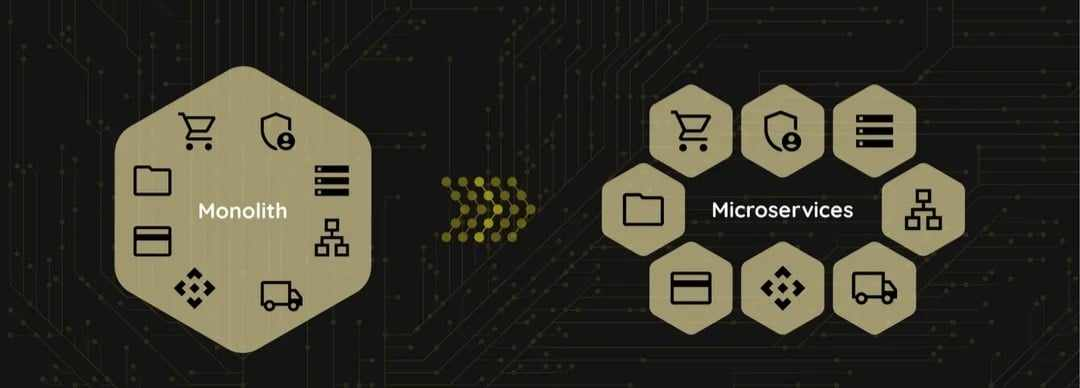
\includegraphics[height = 3cm]{pictures/ChuyenTu_KienTrucNguyenKhoi_Sang_KienTrucViDichVu.jpg}

% % \caption{ViDuHinhAnhTheoChieuDoc}

% \end{figure}

% \begin{figure}[h]

% \centering

% 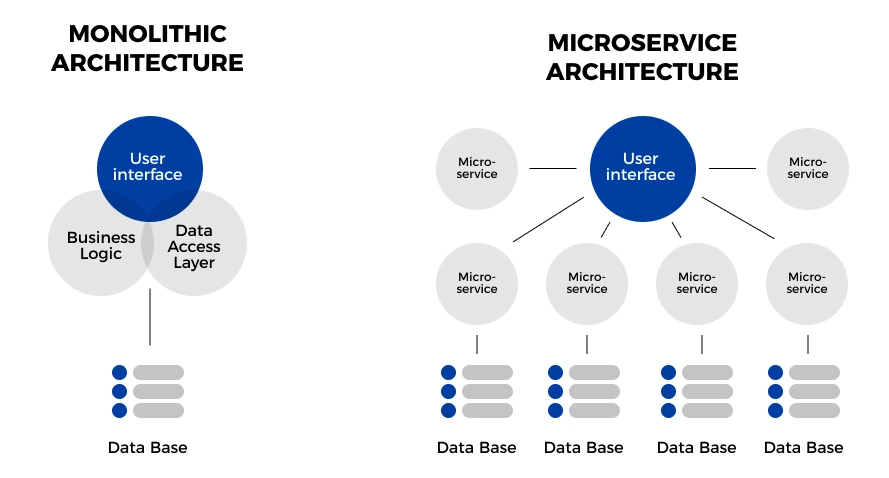
\includegraphics[height = 3cm]{pictures/AnhKhacNhau_KienTrucNguyenKhoi_KienTrucViDichVu.png}

% % \caption{ViDuHinhAnhTheoChieuDoc}

% \end{figure}

% Strangler Fig là chuyển mono sang dịch vụ



% \subsubsection{Một số đặc điểm và ưu điểm của kiến trúc vi dịch vụ}
% Kiến trúc vi dịch vụ có nhiều ưu điểm, đặc biệt với các dự án có quy mô lớn và phức tạp.

\begin{itemize}

    \item Kiến trúc vi dịch vụ phân chia dự án thành các dịch vụ nhỏ.

          \begin{itemize}

              \item Giúp việc phát triển và quản lý hệ thống dễ dàng hơn.

              \item Tận dụng sử dụng tài nguyên theo nhu cầu cho từng dịch vụ riêng.


          \end{itemize}
    \item Các dịch vụ độc lập về nghiệp vụ kinh doanh.
    
    Các nhóm không cần hiểu sâu về mọi khả năng kinh doanh.      Dẫn tới tốc độ phát triển thay đổi nhanh và   tốc độ định giá doanh nghiệp nhanh hơn.
    
    \item Các dịch vụ độc lập về         ngôn ngữ lập trình và CSDL
    \begin{itemize}

        \item     Kiến trúc vi dịch vụ sử dụng đa ngôn ngữ và công nghệ khác nhau. Từ đó tận dụng hiệu quả thế mạnh của từng ngôn ngữ, công nghệ phù hợp nhất cho yêu cầu nghiệp vụ cụ thể.   

        \item        Giảm chi phí và thời gian kiểm thử do ít ràng buộc.
        \item Ví dụ: Mỗi dịch vụ sử dụng ngôn ngữ lập trình nhau khác như: NodeJS, Go, Python, Java, CSharp,...
        
        
        
         
        \begin{figure}[h] 
        \centering
        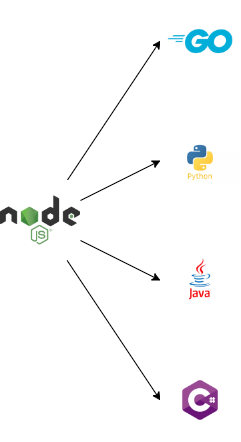
\includegraphics[height=3cm]{pictures/DaNgonNgu/_DaNgonNgu.png}
        \caption{ViDuHinhAnhTheoChieuDoc}  
        % % Thêm vào hình SQL riêng 
        \end{figure} 
        
       


        
        
        


    \end{itemize}
\end{itemize}

%     \item Các  
% 
%                         %     $VD: 




%                           \item Độc lập về     triển khai hệ thống



%                           Mỗi dịch vụ   triển khai độc lập và có thể thực hiện các thay đổi  mà không ảnh hưởng đến các dịch vụ khác.  





%           \end{itemize}
% \end{itemize}

% % Các dịch vụ ít phụ thuộc vào các dịch vụ khác.
% Giảm thiểu ràng buộc và tăng tính linh hoạt của hệ thống.
% Hệ thống có khả năng chịu lỗi cao tăng độ tin cậy.
% % Khả năng phục hồi : Kiến trúc phải được thiết kế để chịu đựng lỗi và các dịch vụ phải có khả năng xử lý lỗi một cách duyên dáng.
% Tính linh hoạt : Kiến trúc phải cho phép phát triển và triển khai nhanh chóng các dịch vụ mới cũng như khả năng thay đổi các dịch vụ hiện có một cách nhanh chóng và dễ dàng.
% \textbf{Từ đó    dễ dàng  mở rộng hệ thống.}
%%%%%%%%%%%%%%%%%%%%%%%%%%%%%%%%%%%%%



%%%%%%%%%%%%%%%%%%%%%%%%%%%%%%%%%%%%%


% Các dịch vụ tương tác với nhau qua hạ tầng mạng.

% Các dịch vụ tương tác với nhau qua hạ tầng mạng.

% Các dịch vụ tương tác với nhau qua hạ tầng mạng.

% Các dịch vụ tương tác với nhau qua hạ tầng mạng.

% Các dịch vụ tương tác với nhau qua hạ tầng mạng.

% Các dịch vụ tương tác với nhau qua hạ tầng mạng.

% Các dịch vụ tương tác với nhau qua hạ tầng mạng.

% Các dịch vụ tương tác với nhau qua hạ tầng mạng.

% Các dịch vụ tương tác với nhau qua hạ tầng mạng.

% \subsubsection{Một số nhược điểm và thách thức của kiến trúc vi dịch vụ}
% % Mặc dù kiến trúc vi dịch vụ có nhiều lợi ích nhưng  cũng có nhiều thách thức:

Chịu ảnh hưởng của đường truyền mạng.
Đồng bộ đồng hồ thời gian.
Ràng buộc về thứ tự sự kiện.
Tính nhất quán và toàn vẹn của dữ liệu.
Khả năng kiểm soát giao dịch.

Giám sát giữa các dịch vụ.
Bảo mật giao tiếp giữa các dịch vụ.


Phát hiện lỗi và sửa lỗi khó khăn, phức tạp hơn.




Chi phí xây dựng, quản lí vận hành lớn. 
 



% \subsubsection{Có thể thêm phần truyền thông trực tiếp, gián tiếp}

% \subsection{Giới thiệu về thiết kế hướng miền}
% Trong quá trình hoạt động kinh doanh, không phải mọi doanh nghiệp đều giữ nguyên mô hình kinh doanh được đưa ra ban đầu của mình. Khi quy mô thị trường thay đổi, việc chuyển đổi mô hình kinh doanh là điều cần thiết. Chuyển đổi kinh doanh như một công cụ linh hoạt giúp các doanh nghiệp có thể phát triển và tồn tại giữa các đối thủ của mình.

Ví dụ:






\begin{itemize}
    \item   Google bắt đầu như một công cụ tìm kiếm trực tuyến, nhưng sau đó đã mở rộng và thay đổi mô hình kinh doanh qua nhiều dịch vụ và sản phẩm khác nhau như: Dịch vụ đám mây Google Cloud Platform, thư điện tử Gmail, bản đồ Google Maps, lưu trữ tập tin Google Drive, \dots
    \item   Amazon từ hiệu sách trực tuyến đã trở thành thị trường cho nhà cung cấp khác như: Thương mại điện tử, Dịch vụ đám mây Amazon Web Services (AWS), \dots
\end{itemize}

\begin{figure}[h]

    \centering

    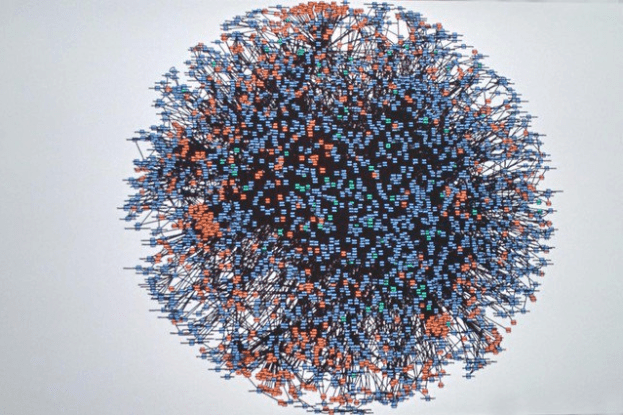
\includegraphics[width = 0.5\textwidth]{pictures/KienTrucViDichVuAmazon/main.png}

    \caption{Kiến trúc vi dịch vụ của Amazon}

\end{figure}


Đối với những doanh nghiệp không chuyển đổi kinh doanh sẽ không thể tồn tại.

Ví dụ: Gần đây, Baemin dịch vụ giao đồ ăn đã rời khỏi thị trường Việt Nam cũng do sức ép từ các đối thủ khác khiến Baemin khó cạnh tranh trong mảng kinh doanh cốt lõi là giao đồ ăn. Các đối thủ này không chỉ cung cấp dịch vụ giao đồ ăn mà còn có đặt xe, giao hàng,...


\begin{figure}[h]
    
    \centering
    
    % ![](pictures/Baemin.png)
    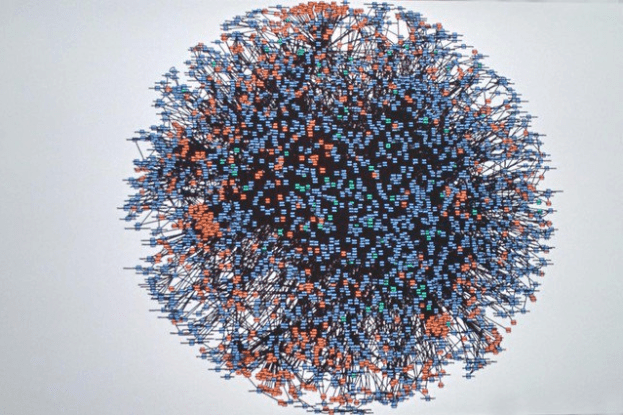
\includegraphics[width = 0.5\textwidth]{pictures/KienTrucViDichVuAmazon/main.png}

    \caption{  Baemin đã rời khỏi thị trường Việt Nam}

\end{figure}

%%%%%%%%%%%%%%%%%%%%%%%%%%%%%%%%%%%%%

% = > Hiện nay, các tổ chức doanh nghiệp có nhu cầu phát triển chuyển đổi kinh doanh để có thể tồn tại và phát triển khi thị trường thay đổi. Từ đó, đáp ứng nhu cầu của khách hàng, giúp mang đến ưu thế cạnh tranh so với các đối thủ. Do đó cần hệ thống chuyển đổi nhanh chóng đáp ứng nhu cầu của dự án và mong đợi của khách hàng.

% = > Kiến trúc vi dịch vụ giải quyết những thách thức và hỗ trợ doanh nghiệp chuyển đổi dễ dàng.

%%%%%%%%%%%%%%%%%%%%%%%%%%%%%%%%%%%%%

Tuy nhiên, để xây dựng được kiến trúc vi dịch vụ tốt cần phải tạo ra các dịch vụ nhỏ phù hợp và duy trì tính độc lập. Nếu không thực hiện đúng các nhóm phụ thuộc lẫn nhau và mất đi lợi thế của kiến trúc vi dịch vụ.

Và từ đó, mẫu thiết kế hướng miền sử dụng để phân tích xây dựng kiến trúc vi dịch vụ.

Thiết kế hướng miền xác định và tổ chức các dịch vụ dựa trên việc hiểu rõ về lĩnh vực kinh doanh, giúp dự án phản ánh đúng các quy trình và quy tắc kinh doanh.

%%%%%%%%%%%%%%%%%%%%%%%%%%%%%%%%%%%%%

% thiết kế hướng miền có thể trợ giúp như thế nào

% Thiết kế hướng miền (thiết kế hướng miền) có thể hỗ trợ kiến trúc và thiết kế kiến trúc vi dịch vụ theo nhiều cách:

% Bối cảnh giới hạn : thiết kế hướng miền nhấn mạnh việc xác định các bối cảnh giới hạn, là các khu vực riêng biệt của miền có ranh giới được xác định rõ ràng. Điều này có thể giúp xác định ranh giới của kiến trúc vi dịch vụ và đảm bảo rằng mỗi kiến trúc vi dịch vụ đều có trách nhiệm rõ ràng và tập trung.

% ngôn ngữ chung : thiết kế hướng miền khuyến khích sử dụng một ngôn ngữ chung được chia sẻ bởi cả chuyên gia ngành và nhân viên kỹ thuật. Điều này có thể giúp đảm bảo rằng các vi dịch vụ giao tiếp hiệu quả với nhau và phù hợp với yêu cầu kinh doanh.

% Ánh xạ bối cảnh: thiết kế hướng miền cung cấp các kỹ thuật để ánh xạ các mối quan hệ giữa các bối cảnh giới hạn. Điều này có thể giúp đảm bảo rằng các vi dịch vụ được thiết kế với sự hiểu biết rõ ràng về sự phụ thuộc của chúng vào các dịch vụ khác.

% Tập hợp: thiết kế hướng miền định nghĩa tập hợp là các cụm đối tượng liên quan cần được coi là một đơn vị nhất quán duy nhất. Điều này có thể giúp đảm bảo rằng các vi dịch vụ được thiết kế với sự hiểu biết rõ ràng về các yêu cầu về tính nhất quán của dữ liệu.

% Tương quan với bối cảnh giới hạn

% Mặc dù người ta thường khuyên nên căn chỉnh ranh giới của kiến trúc vi dịch vụ với ranh giới của bối cảnh giới hạn, nhưng điều đó không phải lúc nào cũng cần thiết hoặc khả thi. Một vi dịch vụ có thể gói gọn nhiều ngữ cảnh giới hạn hoặc một ngữ cảnh giới hạn có thể được phân chia thành nhiều vi dịch vụ, tùy thuộc vào nhu cầu cụ thể của hệ thống và sự cân bằng liên quan. Cuối cùng, mục tiêu là tạo ra một hệ thống mô - đun và có thể bảo trì, đáp ứng các yêu cầu kinh doanh và mối quan hệ giữa bối cảnh giới hạn và các vi dịch vụ phải được thiết kế phù hợp.

% Tương quan với API thực thể

% Nhìn chung, việc thiết kế các vi dịch vụ chỉ dựa trên các hoạt động CRUD của thực thể không được khuyến khích vì nó có thể dẫn đến một kiến trúc liên kết chặt chẽ và không hiệu quả. Các vi dịch vụ phải được thiết kế dựa trên khả năng kinh doanh, có thể phù hợp hoặc không phù hợp với hoạt động CRUD của thực thể.

% thiết kế hướng miền có thể giúp xác định các khả năng kinh doanh và xác định bối cảnh giới hạn, sau đó có thể được sử dụng để hướng dẫn thiết kế các vi dịch vụ. Bằng cách tập trung vào khả năng kinh doanh thay vì hoạt động CRUD thực thể, các vi dịch vụ có thể được liên kết lỏng lẻo hơn, mang tính mô - đun hơn, dễ dàng duy trì và phát triển hơn theo thời gian.



%%%%%%%%%%%
% \section{Yêu cầu nghiệp vụ}
% Yêu cầu nghiệp vụ xác định nội dung, phạm vi, mục tiêu và chức năng mong muốn của hệ thống.

% Nguồn: TCT

% \subsection {Yêu cầu nghiệp vụ của bài toán phụ}
% Trang web "https: //hoadondientu.gdt.gov.vn" là trang web do Tổng Cục Thuế quản lý và sử dụng để thực hiện các quy trình liên quan đến thuế điện tử. Thực tế, yêu cầu đăng ký chính thức từ Tổng Cục Thuế dành cho cá nhân và doanh nghiệp. Vì em không có tài khoản chính thức nên ở đồ án này, em sẽ tạo  tong-cuc-thue-demo - một phiên bản giả lập của hệ thống chính thức, dành cho mục đích học tập phục vụ cho bài toán chính là "Xây dựng kiến trúc vi dịch vụ cho bài toán hóa đơn điện tử".


% \subsubsection{Các chức năng tổng quan của bài toán phụ}
% Để đơn giản hóa bài toán, các chức năng trong đồ án này đã thay đổi so với bài toán thực tế trong tài liệu hướng dẫn sử dụng cổng thông tin điện tử của TCT cho hóa đơn điện tử:

\textbf{Em đã bỏ qua hình thức hóa đơn}

Hóa đơn có mã của cơ quan thuế

Hóa đơn không có mã của cơ quan thuế

\textbf{Bỏ qua các loại hóa đơn khác nhau}

Hóa đơn điện tử giá trị gia tăng

Hóa đơn bán hàng

Hóa đơn bán tài sản công

Hóa đơn bán hàng dự trữ quốc gia

Hóa đơn khác

Phiếu xuất kho kiêm vận chuyển nội bộ

Phiếu xuất kho gửi bán hàng đại lý

\textbf{Bỏ qua phần ký số}

USB Token hay còn gọi là chữ ký số Token là một thiết bị mà mọi doanh nghiệp, tổ chức hiện nay đều cần phải có để thực hiện khai báo và nộp thuế điện tử, cũng như để giao dịch với khách hàng.

\textbf{Bỏ qua phần ký hiệu hóa đơn}

Vì mục đích của ký hiệu hóa đơn là nhóm 6 ký tự thể hiện thông tin về loại hóa đơn điện tử có mã hoặc không mã, năm lập hóa đơn, loại hóa đơn.

\textbf{Bỏ qua chức năng lập hóa đơn điều chỉnh}

E bỏ qua chức năng lập hóa đơn điều chỉnh và chỉ có chức năng lập hóa đơn thay thế.

\textbf{Bỏ qua chức năng phê duyệt hóa đơn}

\textbf{Bỏ qua định dạng file XML,PDF,HTML, EXCEL}

\textbf{Tóm lại, các chức năng tổng quan của tong - cuc - thue - demo bao gồm:}

\underline{\textsc{QUẢN LÝ TÀI KHOẢN}}

Đăng ký

% mail active

% active

Đăng nhập

Đăng xuất

Quên mật khẩu

% mail reset

% reset

Đổi mật khẩu

Thay đổi thông tin

\underline{\textsc{QUẢN LÝ HỆ THỐNG}}

Quản lý vai trò

Quản lý người dùng

\underline{\textsc{QUẢN LÝ DANH MỤC}}

Danh mục khách hàng

Danh mục hàng hóa

\underline{\textsc{QUẢN LÝ HÓA ĐƠN}}

Lập hóa đơn mới

Lập hóa đơn thay thế

Hủy hóa đơn

\underline{\textsc{TRA CỨU HÓA ĐƠN}}

Tra cứu hóa đơn khi NNT chưa đăng nhập

Tra cứu hóa đơn khi NNT đã đăng nhập

\underline{\textsc{GỬI PHẢN HỒI QUA THƯ ĐIỆN TỬ}}

Gửi thông tin của TCT đến NNT
% \subsection{Yêu cầu nghiệp vụ chưa xong}
% \subsection{Yêu cầu nghiệp vụ chưa xong}
% \subsection{Yêu cầu nghiệp vụ chưa xong}
% \subsection{Yêu cầu nghiệp vụ chưa xong}
% \subsection{Yêu cầu nghiệp vụ chưa xong}
% chưa xong
% %@ %@ %@ %@ %@ %@ Mẫu mail

%!<! - - // NNT nhận được thư điện tử của CQT thông báo tiếp nhận tờ khai đăng ký - - >

Trong thời gian 15 phút kể từ khi nhận được tờ khai đăng ký của NNT, Cổng điện tử gửi thư điện tử thông báo về việc tiếp nhận/không tiếp nhận tờ khai đăng ký của NNT.

Nội dung mẫu:

```
Tiêu đề: (TCT Demo) Thông báo về việc tiếp nhận tờ khai đăng ký sử dụng hóa đơn điện tử
Kính gửi: {{Tên NNT}}
Mã số thuế: {{Mã số thuế}}

Căn cứ Tờ khai đăng ký sử dụng hóa đơn điện tử - Ban hành kèm theo Nghị định số 123/2020/NĐ - CP của người nộp thuế (NNT) gửi tới cơ quan thuế ngày {{Ngày nhận}}, cơ quan thuế tiếp nhận Tờ khai đăng ký sử dụng hóa đơn điện tử của NNT, cụ thể như sau:
Tên tờ khai: Tờ khai đăng ký sử dụng hóa đơn điện tử
Mã giao dịch điện tử: {{Mã số thuế + Thời gian}}

Cơ quan thuế thông báo để NNT được biết và thực hiện.
```

%!<! - - NNT nhận được thư điện tử của CQT chấp nhận/không chấp nhận đăng ký sử dụng HĐĐT - - >

Trong thời gian 01 ngày làm việc kể từ ngày Cổng điện tử gửi thông báo về việc tiếp nhận, cơ quan thuế quản lý sẽ gửi thông báo về việc chấp nhận/không chấp nhận đăng ký sử dụng hóa đơn điện tử.

Nội dung mẫu chấp nhận đăng ký sử dụng HĐĐT:

```
Tiêu đề: (TCT Demo) Thông báo về việc chấp nhận đăng ký sử dụng hóa đơn điện tử
Kính gửi: {{Tên NNT}}
Mã số thuế: {{Mã số thuế}}

Sau khi xem xét tờ khai đăng ký sử dụng hóa đơn điện tử của NNT gửi đến cơ quan thuế ngày {{Ngày nhận}}.
Cơ quan thuế thông báo chấp nhận đề nghị đăng ký sử dụng hóa đơn điện tử của NNT.

Cơ quan thuế thông báo để NNT được biết và thực hiện.
```

Nội dung mẫu không chấp nhận đăng ký sử dụng HĐĐT:

```
Tiêu đề: (TCT Demo) Thông báo về việc không chấp nhận đăng ký sử dụng hóa đơn điện tử
Kính gửi: {{Tên NNT}}
Mã số thuế: {{Mã số thuế}}

Sau khi xem xét tờ khai đăng ký sử dụng hóa đơn điện tử của NNT gửi đến cơ quan thuế ngày {{Ngày nhận}}.
Cơ quan thuế thông báo không chấp nhận đề nghị đăng ký sử dụng hóa đơn điện tử của NNT.

Cơ quan thuế thông báo để NNT được biết và thực hiện.
```

%!<! - - NNT nhận được Thông báo tài khoản sử dụng tra cứu HĐĐT trên cổng thông tin điện tử của TCT - - >

Sau khi NNT nhận được thông báo về việc chấp nhận đăng ký sử dụng hóa đơn điện tử, cơ quan thuế gửi thông báo tài khoản sử dụng của NNT qua thư điện tử bao gồm Tên tài khoản và Mật khẩu.

Nội dung mẫu:

```
Tiêu đề: (TCT Demo) Thông báo tài khoản sử dụng tra cứu HĐĐT trên cổng thông tin điện tử của TCT
Kính gửi: {{Tên NNT}}
Mã số thuế: {{Mã số thuế}}

Sau khi xem xét tờ khai đăng ký sử dụng hóa đơn điện tử cơ quan thuế tiếp nhận ngày {{Ngày nhận}}.
Cơ quan thuế thông báo chấp nhận đề nghị đăng ký sử dụng hóa đơn điện tử của NNT và gửi thông tin tài khoản sử dụng tra cứu HĐĐT trên cổng thông tin điện tử của TCT như sau:
Tên tài khoản: {{admin + Mã số thuế}}
Mật khẩu: {{Mật khẩu}}

Cơ quan thuế thông báo để NNT được biết và thực hiện.
```

%!<! - - - - >
%!<! - - - - >
%!<! - - - - >
%!<! - - - - >
%!<! - - - - >
%!<! - - - - >
%!<! - - - - >
%!<! - - - - >
%!<! - - - - >
%!<! - - - - >

%!<! - - NNT nhận được thư điện tử của CQT thông báo tiếp nhận tờ khai đăng ký thay đổi - - >

Trong thời gian 15 phút kể từ khi nhận được tờ khai đăng ký của NNT, Cổng điện tử gửi thư điện tử thông báo về việc tiếp nhận/không tiếp nhận tờ khai đăng ký thay đổi thông tin đăng ký sử dụng của NNT.

Nội dung mẫu:

```
Tiêu đề: (TCT Demo) Thông báo về việc tiếp nhận tờ khai đăng ký thay đổi thông tin đăng ký sử dụng của NNT
Kính gửi: {{Tên NNT}}
Mã số thuế: {{Mã số thuế}}

Căn cứ Tờ khai đăng ký thay đổi thông tin đăng ký sử dụng của NNT gửi tới cơ quan thuế ngày {{Ngày nhận}}, cơ quan thuế tiếp nhận Tờ khai đăng ký sử dụng hóa đơn điện tử của NNT, cụ thể như sau:
Tên tờ khai: Tờ khai đăng ký thay đổi thông tin đăng ký sử dụng của NNT
Mã giao dịch điện tử: {{Mã số thuế + Thời gian}}

Cơ quan thuế thông báo để NNT được biết và thực hiện.
```

%!<! - - NNT nhận được thư điện tử của CQT chấp nhận/không chấp nhận đăng ký sử dụng HĐĐT - - >

Trong thời gian 01 ngày làm việc kể từ ngày Cổng điện tử gửi thông báo về việc tiếp nhận, cơ quan thuế quản lý sẽ gửi thông báo về việc chấp nhận/không chấp nhận đăng ký thay đổi thông tin đăng ký sử dụng của NNT.

Nội dung mẫu chấp nhận đăng ký thay đổi thông tin đăng ký sử dụng của NNT

```
Tiêu đề: (TCT Demo) Thông báo về việc chấp nhận đăng ký thay đổi thông tin đăng ký sử dụng của NNT
Kính gửi: {{Tên NNT}}
Mã số thuế: {{Mã số thuế}}

Sau khi xem xét tờ khai đăng ký thay đổi thông tin đăng ký sử dụng của NNT gửi đến cơ quan thuế ngày {{Ngày nhận}}.
Cơ quan thuế thông báo chấp nhận đề nghị đăng ký thay đổi thông tin đăng ký sử dụng của NNT.

Cơ quan thuế thông báo để NNT được biết và thực hiện.
```

Nội dung mẫu không chấp nhận đăng ký thay đổi thông tin đăng ký sử dụng của NNT

```
Tiêu đề: (TCT Demo) Thông báo về việc không chấp nhận đăng ký thay đổi thông tin đăng ký sử dụng của NNT
Kính gửi: {{Tên NNT}}
Mã số thuế: {{Mã số thuế}}

Sau khi xem xét tờ khai đăng ký thay đổi thông tin đăng ký sử dụng của NNT gửi đến cơ quan thuế ngày {{Ngày nhận}}.
Cơ quan thuế thông báo không chấp nhận đề nghị đăng ký thay đổi thông tin đăng ký sử dụng của NNT.

Cơ quan thuế thông báo để NNT được biết và thực hiện.
```

%!<! - - - - >
%!<! - - - - >
%!<! - - - - >
%!<! - - - - >
%!<! - - - - >
%!<! - - - - >
%!<! - - - - >

%!<! - - Sau khi gửi yêu cầu lấy lại mật khẩu NNT sẽ nhận được thông báo của CQT qua gửi thư điện tử - - >

Nội dung mẫu:

```
Tiêu đề: (TCT Demo) Thông báo về việc lấy lại mật khẩu
Kính gửi: {{Tên NNT}}
Mã số thuế: {{Mã số thuế}}

Sau khi xem xét yêu cầu lấy lại mật khẩu của NNT gửi đến cơ quan thuế ngày {{Ngày nhận}}.
Cơ quan thuế gửi thông tin tài khoản sử dụng tra cứu HĐĐT trên cổng thông tin điện tử của TCT như sau:
Tên tài khoản: {{Tên tài khoản}}
Mật khẩu mới: {{Mật khẩu mới}}

Cơ quan thuế thông báo để NNT được biết và thực hiện.
```

%@ %@ %@ Chi tiết các chức năng của TCT Demo:

Chi tiết các chức năng của TCT Demo:

QUẢN LÝ TÀI KHOẢN

Quản lý tài khoản là một chức năng phổ biến trong nhiều ứng dụng. Chức năng này đảm bảo tính bảo mật và an toàn trong việc sử dụng tài khoản.

%!<! - - Chức năng: "Đăng ký sử dụng hóa đơn điện tử" - - >

NNT nhập MST có 10 ký tự cho cá nhân, doanh nghiệp hoặc 14 ký tự cho chi nhánh của doanh nghiệp với định dạng "Mã số thuế doanh nghiệp - Mã chi nhánh".
Ví dụ:
Mã số thuế 10 ký tự: 0123456789
Mã số thuế 14 ký tự: 0123456789 - 001

Hệ thống tự động hiển thị thông tin Đăng ký thuế của NNT bao gồm "Tên của NNT", "Mã cơ quan thuế quản lý" và "Tên cơ quan thuế quản lý".

Tiếp theo, NNT nhập các thông tin hợp lệ: "Người liên hệ", "Điện thoại liên hệ", "Địa chỉ liên hệ", "Thư điện tử".

Cuối cùng, NNT gửi đăng ký với thông tin "Ngày thực hiện" là ngày NNT đang đăng ký hóa đơn điện tử.

Sau khi gửi thông tin đăng kí NNT sẽ nhận được thông báo làm việc của CQT qua gửi thư điện tử về việc tiếp nhận và chấp nhận đăng ký, cùng với tài khoản và mật khẩu cho NNT.

%!<! - - // Nếu mã số thuế không đúng định dạng, hệ thống sẽ thông báo: "Mã số thuế phải có độ dài 10 hoặc 14 ký tự và đúng định dạng". - - >
%!<! - - // Nếu mã số thuế tồn tại, hệ thống kiểm tra xem NNT đã đăng ký sử dụng hóa đơn điện tử khác chưa. Nếu đã tồn tại tờ khai đăng ký, hệ thống thông báo: "Đã tồn tại tờ khai đăng ký sử dụng hóa đơn điện tử khác của NNT đã được cơ quan thuế chấp nhận". - - >

%!<! - - // Người liên hệ: phải chứa một chuỗi kí tự và không được để trống. - - >
%!<! - - // Điện thoại liên hệ: phải chứa một chuỗi kí tự số và dấu " + " ở đầu chuỗi (nếu có) và không được để trống. - - >
%!<! - - // Địa chỉ liên hệ: phải chứa một chuỗi kí tự và không được để trống. - - >
%!<! - - // Thư điện tử: phải chứa một chuỗi kí tự có định dạng email và không được để trống. - - >

%!<! - - // Khi NNT nhấn nút "Ký gửi", hệ thống sẽ hiển thị thông báo hỏi "Xác nhận ký gửi" với hai lựa chọn là "Đồng ý" hoặc "Hủy bỏ". - - >
%!<! - - // Nếu NNT chọn "Đồng ý", hệ thống sẽ thông báo: "Gửi thông tin đăng ký sử dụng hóa đơn điện tử cho cơ quan thuế thành công". - - >

%!<! - - - - >
%!<! - - Chức năng: "Thay đổi đăng ký sử dụng hóa đơn điện tử" - - >

Trong quá trình sử dụng hóa đơn điện tử, khi NNT muốn thay đổi đăng ký sử dụng hóa đơn, họ có thể sử dụng chức năng "Thay đổi đăng ký sử dụng hóa đơn điện tử".

NNT Nhập thông tin có thể thay đổi, bao gồm: Tên NNT, Người liên hệ, Điện thoại liên hệ, Địa chỉ liên hệ, Thư điện tử.
Cuối cùng, NNT gửi đăng ký thay đổi với thông tin "Ngày thực hiện" là ngày NNT đang đăng ký thay đổi hóa đơn điện tử.

Sau khi gửi thông tin thay đổi đăng ký, NNT sẽ nhận được thông báo làm việc từ cơ quan thuế qua thư điện tử về việc tiếp nhận và chấp nhận thay đổi đăng ký cho NNT.

%!<! - - Chức năng: "Đăng nhập tài khoản" - - >

Sau khi CQT gửi thư điện tử chứa tài khoản và mật khẩu cho NNT, NNT thực hiện nhập đầy đủ thông tin bao gồm: Tên đăng nhập, Mật khẩu để thực hiện việc đăng nhập vào tài khoản.

%!<! - - Chức năng: "Đăng xuất tài khoản" - - >

Chức năng để NNT đăng xuất tài khoản.

%!<! - - Chức năng: "Đổi mật khẩu" - - >

NNT cung cấp đầy đủ thông tin bao gồm: Mật khẩu cũ, Mật khẩu mới và Nhập lại mật khẩu mới để thực hiện việc thay đổi mật khẩu.

%!<! - - Chức năng: "Quên mật khẩu" - - >

NNT cung cấp đầy đủ thông tin bao gồm: Tên đăng nhập, Thư điện tử. Sau đó, nhấn "Quên mật khẩu" để khôi phục mật khẩu. CQT gửi mật khẩu mới về email của NNT.

%!<! - - QUẢN LÝ HỆ THỐNG - - >

%!<! - - Chức năng: "Quản lý vai trò" - - >

Người quản trị hệ thống (admin) là một vai trò cố định được phép sử dụng tất cả các chức năng trên Cổng điện tử.
Người quản trị hệ thống có thể thực hiện CRUD "Vai trò" với các thông tin bao gồm: "ID", "Tên vai trò" và "Quyền".

Các quyền bao gồm:
Thay đổi đăng ký sử dụng hóa đơn điện tử
Quản lý vai trò
Quản lý người dùng
Quản lí danh mục
Quản lí hóa đơn
Tra cứu hóa đơn

%!<! - - Chức năng: "Quản lý người dùng" - - >

Người quản trị hệ thống có thể thực hiện CRUD "Người dùng" với các thông tin bao gồm: "Tên người dùng", "Mật khẩu", "Điện thoại", "Thư điện tử" và "Vai trò".

%!<! - - QUẢN LÝ DANH MỤC - - >

%!<! - - Chức năng: "Danh mục khách hàng" - - >

Chức năng này thực hiện CRUD "Khách hàng" có các thông tin: "Mã khách hàng", "Tên khách hàng", "Mã số thuế", "Tên NNT", "Địa chỉ", "SĐT khách hàng", Số tài khoản, Ngân hàng

%!<! - - Chức năng: "Danh mục hàng hóa" - - >

Chức năng này thực hiện CRUD "Hàng hóa" có các thông tin: "Mã hàng hóa, dịch vụ", "Tên hàng hóa, dịch vụ", "Đơn vị tính", "Đơn giá", "Thuế suất".

%!<! - - QUẢN LÝ HÓA ĐƠN ĐIỆN TỬ - - >

%!<! - - Chức năng: "Lập hóa đơn mới" - - >

Nhập thông tin người bán: MST người bán, Tên người bán, Địa chỉ người bán, Số điện thoại người bán.

Nhập thông tin người mua: Mã khách hàng, Tên khách hàng, Mã số thuế, Địa chỉ khách hàng, SĐT khách hàng.

Nhập thông tin hàng hóa, dịch vụ: "Số thứ tự", "Mã hàng hóa, dịch vụ", "Tên hàng hóa, dịch vụ", "Đơn vị tính", "Đơn giá", "Thuế suất" và "Số lượng".

Hệ thống tự động tính toán:

- Ngày lập hóa đơn sẽ tự động là ngày hiện tại khi người lập tạo hóa đơn mới.

- Tổng tiền trước thuế.

- Tổng tiền sau thuế.

%!<! - - Chức năng: "Lập hóa đơn thay thế" - - >

Chức năng này cho phép thay đổi các thông tin trong hóa đơn gốc.

Lưu ý:

- Hãy lưu trữ thông tin ID của hóa đơn thay thế trong trạng thái "Bị thay thế" của hóa đơn gốc.

- Hãy lưu trữ thông tin ID của hóa đơn gốc trong trạng thái "Thay thế" của hóa đơn thay thế.

%!<! - - Chức năng: "Hủy hóa đơn" - - >

Chức năng này cho phép xóa hóa đơn và các hóa đơn thay thế liên quan.

%!<! - - TRA CỨU HÓA ĐƠN - - >

Người sử dụng có thể thực hiện tra cứu hóa đơn trên cổng thông tin điện tử theo 2 cách:
Cách 1: Tra cứu hóa đơn khi NNT chưa đăng nhập
Cách 2: Tra cứu hóa đơn khi NNT đã đăng nhập

%!<! - - Chức năng: "Tra cứu hóa đơn khi NNT chưa đăng nhập" - - >

%!<! - - Tra cứu thông tin hóa đơn - - >

Người tra cứu nhập thông tin bao gồm: Mã số thuế người bán, Số hóa đơn, Tổng tiền thuế, Tổng tiền thanh toán, Ngày lập hóa đơn.

%!<! - - Kết quả: - - >
%!<! - - - Nếu hóa đơn điện tử không hợp lệ, hệ thống sẽ hiển thị thông báo: "Không tồn tại hóa đơn có thông tin trùng khớp với các thông tin tổ chức, cá nhân tìm kiếm”. - - >
%!<! - - - Nếu hóa đơn điện tử hợp lệ, hệ thống sẽ hiển thị thông báo: "Tồn tại hóa đơn có thông tin trùng khớp với các thông tin tổ chức, cá nhân tìm kiếm". - - >
%!<! - - - Nếu hóa đơn tìm kiếm là hóa đơn thay thế, bị thay thế hệ thống sẽ hiển thị thông tin bổ sung về hóa đơn liên quan: "Hóa đơn này là hóa đơn thay thế cho hóa đơn có ID: {{ID}}" hoặc "Hóa đơn này là hóa đơn bị thay thế của hóa đơn có ID: {{ID}}". - - >

%!<! - - Tra cứu thông tin "Mã số thuế" - - >

Người tra cứu nhập thông tin bao gồm: Mã số thuế.

%!<! - - Kết quả: - - >
%!<! - - - Nếu đã đăng kí, hệ thống sẽ hiển thị thông báo: “MST 0107001729 đã đăng ký sử dụng hóa đơn điện tử theo Nghị định 123/2020/NĐ - CP". - - >
%!<! - - - Nếu NNT chưa đăng kí hoặc đã đăng kí nhưng cơ quan thuế có thông báo về việc không được chấp nhận đăng kí sử dụng hóa đơn điện tử, hệ thống sẽ hiển thị thông báo: “MST 0107001728 chưa sử dụng hóa đơn điện tử theo Nghị định 123/2020/NĐ - CP". - - >
%!<! - - Chức năng: "Tra cứu hóa đơn khi NNT đã đăng nhập" - - >

Cổng điện tử hỗ trợ tra cứu 2 loại hóa đơn là hóa đơn bán ra và hóa đơn mua vào.

Người tra cứu nhập thông tin tra cứu bao gồm: Mã số thuế người bán, Ngày lập hóa đơn và Số hóa đơn.

Cổng điện tử hỗ trợ các chức năng sau: Xem thông tin hóa đơn, In hóa đơn và Xuất hóa đơn (định dạng Excel, XML, PDF).

%!<! - - GỬI PHẢN HỒI QUA THƯ ĐIỆN TỬ - - >

%!<! - - - Gửi thông tin làm việc của TCT cho yêu cầu của NNT - - >

%!<! - - $ NNT nhận được thư điện tử của CQT thông báo tiếp nhận tờ khai đăng ký - - >

%!<! - - $ NNT nhận được thư điện tử của CQT chấp nhận/không chấp nhận đăng ký sử dụng HĐĐT - - >

%!<! - - $ NNT nhận được Thông báo tài khoản sử dụng tra cứu HĐĐT trên cổng thông tin điện tử của TCT - - >

%!<! - - $ NNT nhận được thư điện tử của CQT thông báo tiếp nhận tờ khai đăng ký thay đổi - - >

%!<! - - $ NNT nhận được thư điện tử của CQT chấp nhận/không chấp nhận đăng ký sử dụng HĐĐT - - >
%!<! - - Yêu cầu nghiệp vụ của bài toán chính - - >

%!<! - - Các chức năng của bài toán chính - - >

%!<! - - THÔNG BÁO - - >

Chức năng CRUD "Thông báo" bao gồm các thông tin: ID, tiêu đề, nội dung, thời gian.

%!<! - - QUẢN LÝ TÀI KHOẢN - - >

Tương tự " TCT Demo" với các chức năng sau:

Đăng ký
Đăng nhập
Đăng xuất
Quên mật khẩu
Xem thông tin
Thay đổi thông tin
Đổi mật khẩu

%!<! - - CẤU HÌNH EMAIL - - >

Cấu hình bao gồm:

Địa chỉ email
Mật khẩu email

Loại email gửi:

Xác nhận tài khoản mới
Quên mật khẩu
Gửi thông tin hóa đơn cho khách hàng

%!<! - - QUẢN LÝ DANH MỤC - - >

Tương tự " TCT Demo" bao gồm:

Danh mục khách hàng
Danh mục hàng hóa

%!<! - - QUẢN LÝ HỆ THỐNG - - >

Tương tự " TCT Demo" nhưng có thêm quyền "Cấu hình Email".

%!<! - - QUẢN LÝ HÓA ĐƠN ĐIỆN TỬ - - >

Tương tự " TCT Demo"

%!<! - - TRA CỨU HÓA ĐƠN - - >

Có 3 cách tra cứu:

Tra cứu 1 hóa đơn theo "Mã hóa đơn"
Tra cứu tất cả hóa đơn bán ra
Tra cứu tất cả hóa đơn mua vào

%!<! - - BÁO CÁO VÀ PHÂN TÍCH HÓA ĐƠN - - >

Các chức năng bao gồm:

Số lượng hóa đơn đã sử dụng
Tổng tiền trước thuế
Tổng tiền sau thuế
Tổng số tiền thuế
Số lượng khách hàng
Số lượng sản phẩm

%@ %@ %@ Tự động

Nghiệp vụ của bài toán chính
Các chức năng của bài toán chính
THÔNG BÁO
CRUD thông báo có (id, tiêu đề, nội dung, thời gian)
TÀI KHOẢN
Sử dụng tài khoản của " TCT Demo" với các chức năng tương tự Đăng ký, Đăng nhập, Đăng xuất, Quên mật khẩu, Xem thông tin, Thay đổi thông tin, Đổi mật khẩu
CẤU HÌNH EMAIL ĐỂ GỬI HÓA ĐƠN CHO KHÁCH HÀNG

Địa chỉ email
Mật khẩu email
CHỨC NĂNG DANH MỤC
Giống với " TCT Demo" gồm "Danh mục khách hàng" và "Danh mục hàng hóa"
TRA CỨU HÓA ĐƠN:
Có 3 cách tra cứu:
Tra cứu 1 hóa đơn theo "Mã hóa đơn".
Tra cứu tất cả hóa đơn bán ra.
Tra cứu tất cả hóa đơn mua vào.
BÁO CÁO VÀ PHÂN TÍCH HÓA ĐƠN

Số lượng hóa đơn đã sử dụng
Tổng trước thuế
Tổng sau thuế
Tổng số tiền thuế
Số lượng khách hàng
Số lượng sản phẩm

%!<! - - - - >
%!<! - - Phân quyền - - >
%!<! - - Thay đổi - - >
%!<! - - Lập hóa đơn mới - - >
%!<! - - Tra cứu - - >
%!<! - - mail - - >

%@ %@ %@ 4. Các sơ đồ phân tích thiết kế hệ thống

%@ %@ %@ %@ %@ %@ 4.1. UML Use Case Diagrams

%@ %@ %@ %@ %@ %@ 4.2. UML Activity Diagrams

%@ %@ %@ %@ %@ %@ 4.3. UML Sequence Diagrams

%@ %@ %@ %@ %@ %@ 4.4. UML Class Diagrams


\section{Chi tiết và áp dụng thiết kế hướng miền}
% https:// thiết kế hướng miền - practitioners.com/home/glossary
% https: //www.infoq.com/minibooks/domain - driven - design - quickly
\subsection{Đôi nét về thiết kế hướng miền}
\newpage
\begin{center}
{\bfseries NHẬN XÉT CỦA GIẢNG VIÊN HƯỚNG DẪN}
\end{center}
1.	Mục đích và nội dung của đồ án:

\vspace{4ex} % Thêm khoảng cách dọc

2.	Kết quả đạt được:

3.	Ý thức làm việc của sinh viên:

Hà Nội, \today

\textbf{Giảng viên hướng dẫn}

\textit{(Ký và ghi rõ họ tên)}

\newpage


% \newpage
\begin{center}
{\bfseries NHẬN XÉT CỦA GIẢNG VIÊN HƯỚNG DẪN}
\end{center}
1.	Mục đích và nội dung của đồ án:

\vspace{4ex} % Thêm khoảng cách dọc

2.	Kết quả đạt được:

3.	Ý thức làm việc của sinh viên:

Hà Nội, \today

\textbf{Giảng viên hướng dẫn}

\textit{(Ký và ghi rõ họ tên)}

\newpage


% Hai vấn đề cốt lõi được giải quyết bằng thiết kế hướng miền:
% 1. Thiết kế, phân chia cơ cấu doanh nghiệp như thế nào cho hợp lý?
% 2. Kiến trúc kỹ thuật có phù hợp với kiến trúc kinh doanh không?
% %
% Yêu cầu nghiệp vụ của từng sub
% %
% Sơ đồ if else Đ S
% %
% sub trước model
% %
%%%%%%%%%%%%%%%%%%%%%%%%%%%%%%%%%%%%%
\end{document}

\section{xxxxxxx}
\subsection{xxxxxxx}
\subsubsection{xxxxxxx}
\newpage
\begin{center}
{\bfseries NHẬN XÉT CỦA GIẢNG VIÊN HƯỚNG DẪN}
\end{center}
1.	Mục đích và nội dung của đồ án:

\vspace{4ex} % Thêm khoảng cách dọc

2.	Kết quả đạt được:

3.	Ý thức làm việc của sinh viên:

Hà Nội, \today

\textbf{Giảng viên hướng dẫn}

\textit{(Ký và ghi rõ họ tên)}

\newpage


% phải có CQRS (Phân chia trách nhiệm truy vấn lệnh)

CQRS là một mẫu kiến trúc riêng biệt có thể được sử dụng kết hợp với thiết kế hướng miền để đạt được những lợi ích nhất định, chẳng hạn như cải thiện hiệu suất và khả năng mở rộng. Tuy nhiên, nó không phải là một yêu cầu để triển khai thiết kế hướng miền.

% phải có event
Ngôn ngữ chung (Ubiquitous Language)